\chapter{Machine Learning for Speech}\label{ch:machine_learning}
The goal for this chapter is to understand different kinds of Artificial Neural Network (ANN), starting with a historical overview of older, but highly recognized machine learning techniques still used today. After the brief overview, ANN will be looked at in more detail and different configurations are shown. Leading on, a simple description on TensorFlow and respective APIs (with example code) is done in order to understand future code development. Finally, ending the chapter with a small comparison study to get a feeling for the different parameter values.

\section{Historical Overview}
The following section will encapsulate different methods that 
can be used in the field of speech processing and recognition.
Starting with statistical models and mapping algorithms,
further leading to knowledge-based systems that render greater
efficiency when large data sets are available.

\subsubsection{Hidden Markov Model}

The forward and backward recursions used in HMM  were
created by Ruslan L. Stratonovich in 1960
\cite{stratonovich1960conditional}.
It is the most successfully used pattern recognition technique used for speech recognition.
In contrast to knowledge-based approaches, this model has
a strong and secure mathematical foundation
where a mathematical model is signalized on the Markov
Model and a set of output distribution. Speech is divided
into smaller audible samples where each sample represents a state in the Markov Model. 
By the probabilities of transition, there will be a shift from one state to another
\cite[p.~2]{gaikwad2010review}\cite{togneri1990speech}.

\subsubsection{Dynamic Time Warping}

Dynamic Time Warping (DTW) is an algorithm that compares words with pre-given reference words.
It measures the patterns between two sequences that will vary in time or speed.\cite{togneri1990speech}
To output speech, the algorithm tries to alter the time variable of the unknown speech until it matches one of the reference words.

\subsubsection{Vector Quantization}

Vector Quantization (VQ) is used to map vectors from a big vector space to a finite region in space. 
It needs compact code-blocks for reference models and codebook searcher in place of more costly evaluation methods. 
Each word receives a VQ codebook that is based on repeated sequences of the word.
The test data is evaluated on all codebooks and the automated speech recognizer picks the codebook with the lowest distance measured
\cite[p.~20-21]{togneri1990speech}.


\section{Artificial Neural Networks}\label{sec:ANN}
%---------------------------------------------------
\subsection{What is an Artificial Neural Network?}
Artificial Neural Networks are nothing but a computerized representation of the human brain. 
They have the ability to acquire and maintain knowledge (information based) and can be defined as a set of processing units, represented by artificial neurons,
interlinked by a lot of interconnections
(artificial synapses) \cite[p.~5]{Silva2016}.\\\\
The human brain learns from its experiences, creating new neural pathways. These interconnected chains of neurons are stronger than others and can be modulated, or changed,
following learning or during behavioural modifications.
The strength of a neural connection is given by a weighted value, called synaptic weights.

\subsection{Artificial Neuron}
The Artificial neuron is the processing unit of an artificial neural network, which is a simplified model of the biological neuron.
This model was inspired by the analysis of how a cell membrane of a neuron generates and propagates electrical impulses (Hodgkin and Huxley 1952) \cite[p.~11]{Silva2016}.
The purpose of artificial neurons is to simulate the basic function of biological ones,
which are typically comprised of four parts:
\begin{enumerate}
    \item Dendrites: Accept inputs
    \item Soma(Cell body): Process the inputs
    \item Axon: Turn the processed inputs into outputs
    \item Synapses: The electrochemical connections between neurons 
\end{enumerate}
Figure \ref{fig:AN} illustrates the four main functions of a biological neuron, represented by the artificial one.\\\\
The artificial neurons used in artificial neural networks are non-linear, usually providing continuous outputs,
and performing simple functions,
such as gathering signals available on their inputs,
assembling them according to their operational functions,
and producing a response considering their innate activation functions \cite[p.~11]{Silva2016}. 
\begin{figure}[H]
\centering
    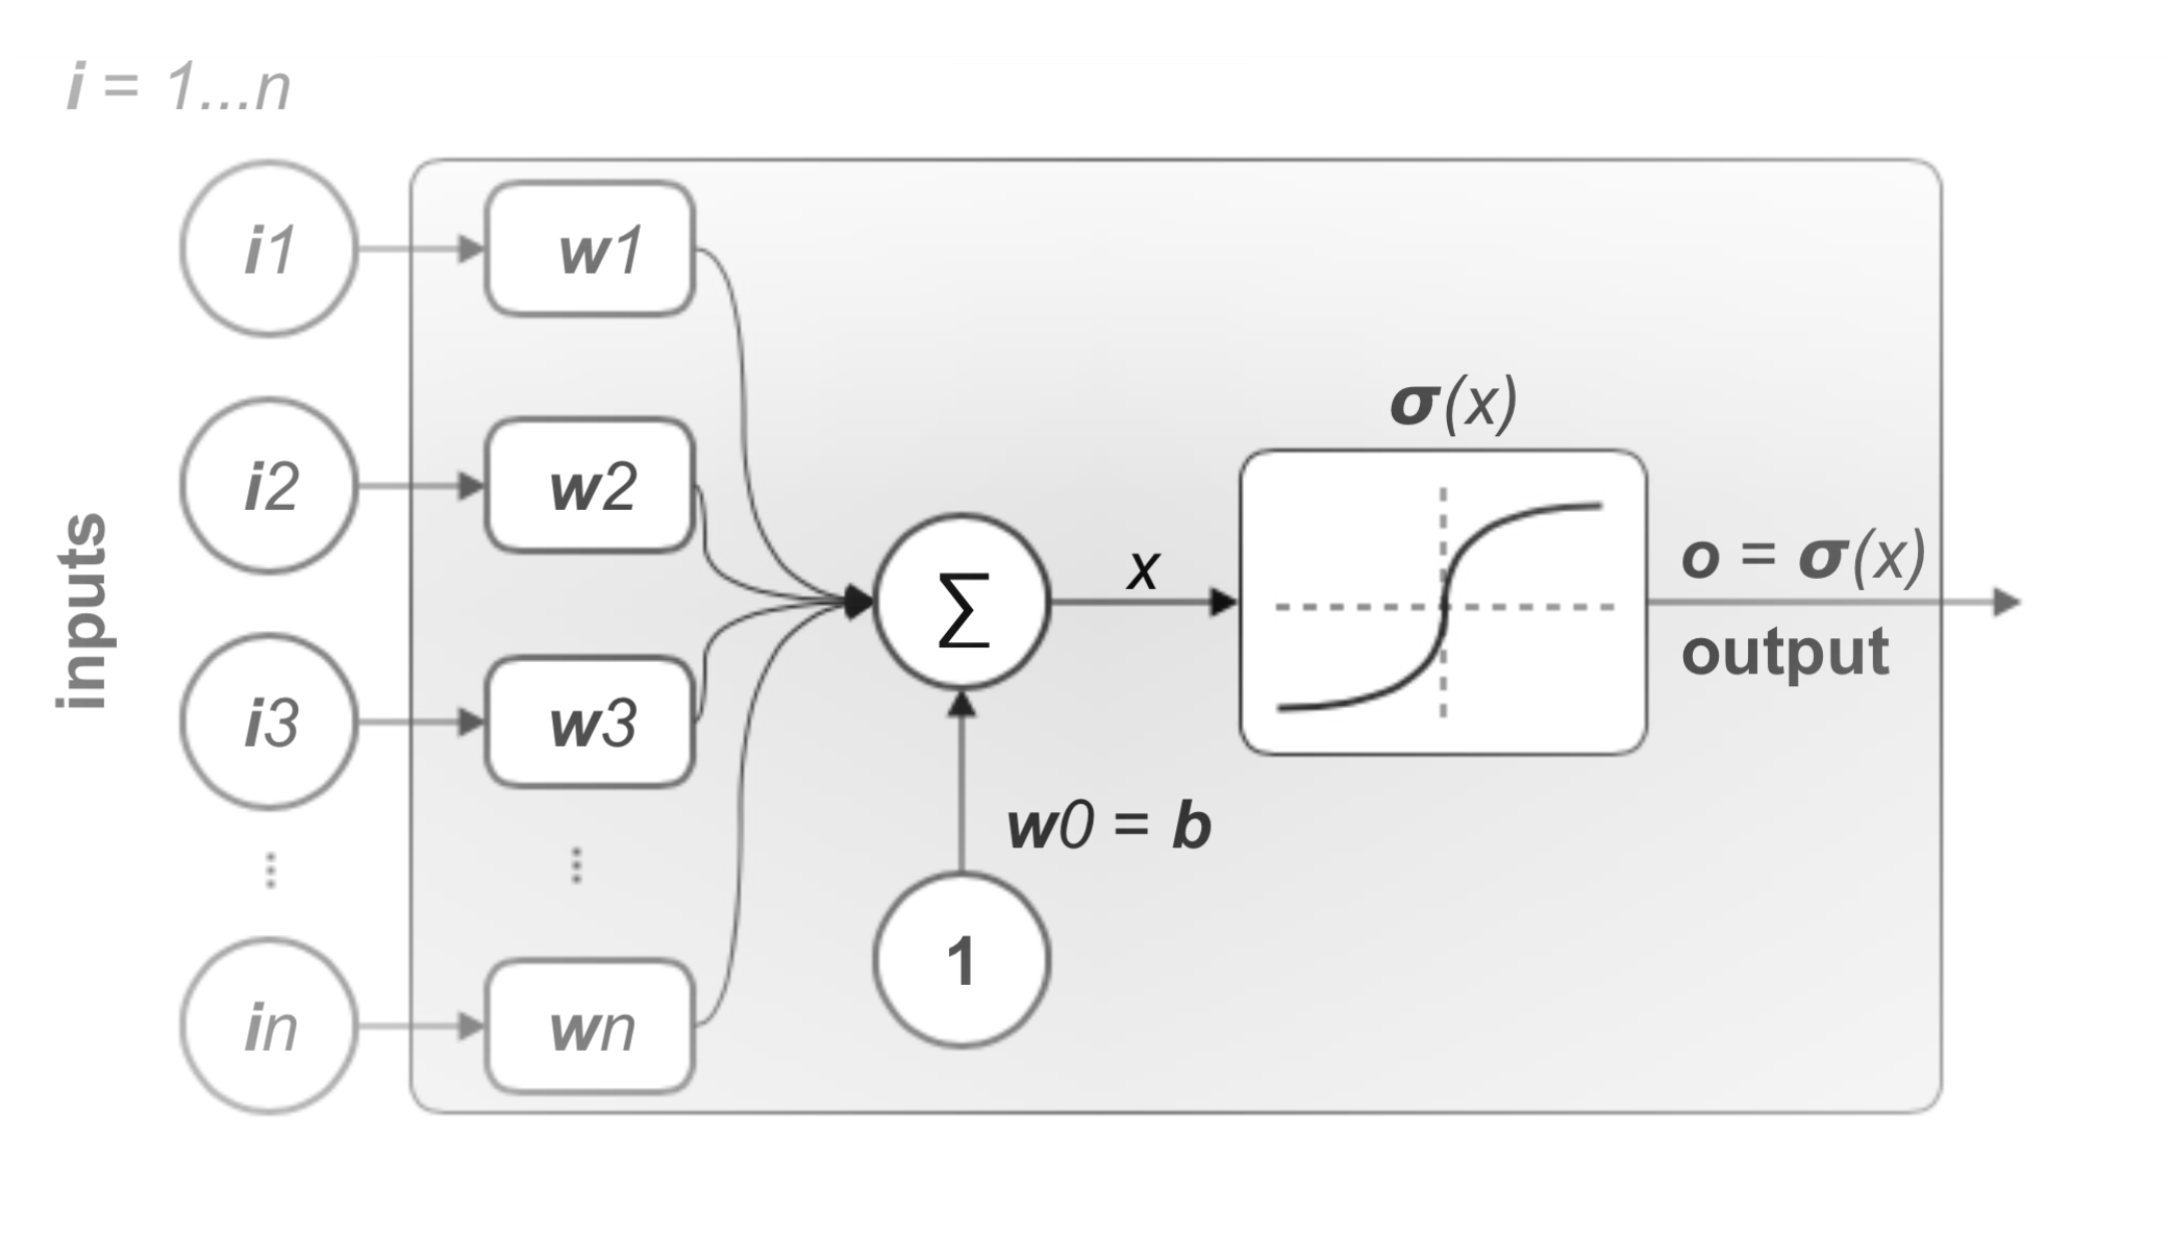
\includegraphics[width=0.75\textwidth]
    {machine_learning/00_Artificial_Neuron}
    \caption{The artificial neuron.}
    \label{fig:AN}
\end{figure}
Each neuron from a network can be implemented as shown in Fig.
\ref{fig:AN}. The multiple input signals coming from the external environment are represented by the set
$\left\{i_1,i_2,i_3,...,i_n \right\}$, analogous to the electrical signals received by the dendrites from the biological neuron.\\\\
Those inputs are then multiplied with a weight vector
$\left\{w_1,w_2,w_3,...,w_n \right\}$. 
This is how each input gains a different relevance that will affect the output of the neuron.
From $x$, it can be seen that the neuron computes a weighted sum of all its weights and biases, which they are passed onto the activation function to be mapped, analogous to the biological
basic function of the Soma and Axon respectively.
This process is repeated for each neuron found in any layer of a neural network.

%---------------------------------------------------
\section{Types of Artificial Neural Networks}
%---------------------------------------------------
\subsection{Feed forward Network}
This type of simple neural network is comprised of one input
layer and one neural layer, which also acts as the output layer.
The flow of information is unidirectional, starting from the input layer and progressing to the output layer. As such, the number of outputs from the neural network will always coincide with the number of neurons in the network.
These networks are usually employed in
pattern classification and linear filtering problems. 
The Perceptron and the ADALINE architectures are among the most recognized feed-forward neural networks and they work well with Hebb's rule and the Delta rule for training.

\subsection{Deep Recurrent Neural Network}
To explain how a deep recurrent neural network (RNN) looks like first we will see what a deep neural network is made of and after that, the recurrent part will be added to form a more complex and powerful network.\\\\
Networks with multiple layers have one or more hidden neural layers. Such a network will always have one input layer with multiple samples and a series of variable layers.
In contrast to the simple feed-forward network, these hidden layers are not constrained to have the same size as the input layer. This means
that the size can depend on the complexity of the problem being
tackled by the network, as well as the quantity and quality of the available data. The last layer still occupies a double role as both a neuron layer and output layer.\\\\
Another key element is the fact that the outputs of the neurons are used for feedback inputs to the other neurons.
This feature makes the network great for time-variant systems where the new outputs can benefit from the previous information.

\subsection{Long Short-Term Memory}\label{sub:LSTM}
Long Short-Term Memory networks, for short “LSTMs”, are a special case of the recurrent neural network, that is capable of learning long-term dependencies.
Firstly used in 1997 by Sepp Hochreiter and Jürgen Schmidhuber
 \cite{Father} and refined by Felix Gers and his team
 \cite{Gers99learningto}.
Nowadays, after further refinement,
LSTMs work incredibly well on various problems and give better results for most problems that require RNNs.
They remember information for long periods of time by default, making them the perfect fit to avoid long-term dependency problems.\\\\
LSTMs have a chain-like structure of four layers, with repeating modules that interact in specific ways. For simplicity, in the following explanation of the internal states of an LSTM, the input $X$ will represent the normal input to the network concatenated with the previous state, $X = x_i | h_{t-1}$.
\begin{figure}[H]
\centering
    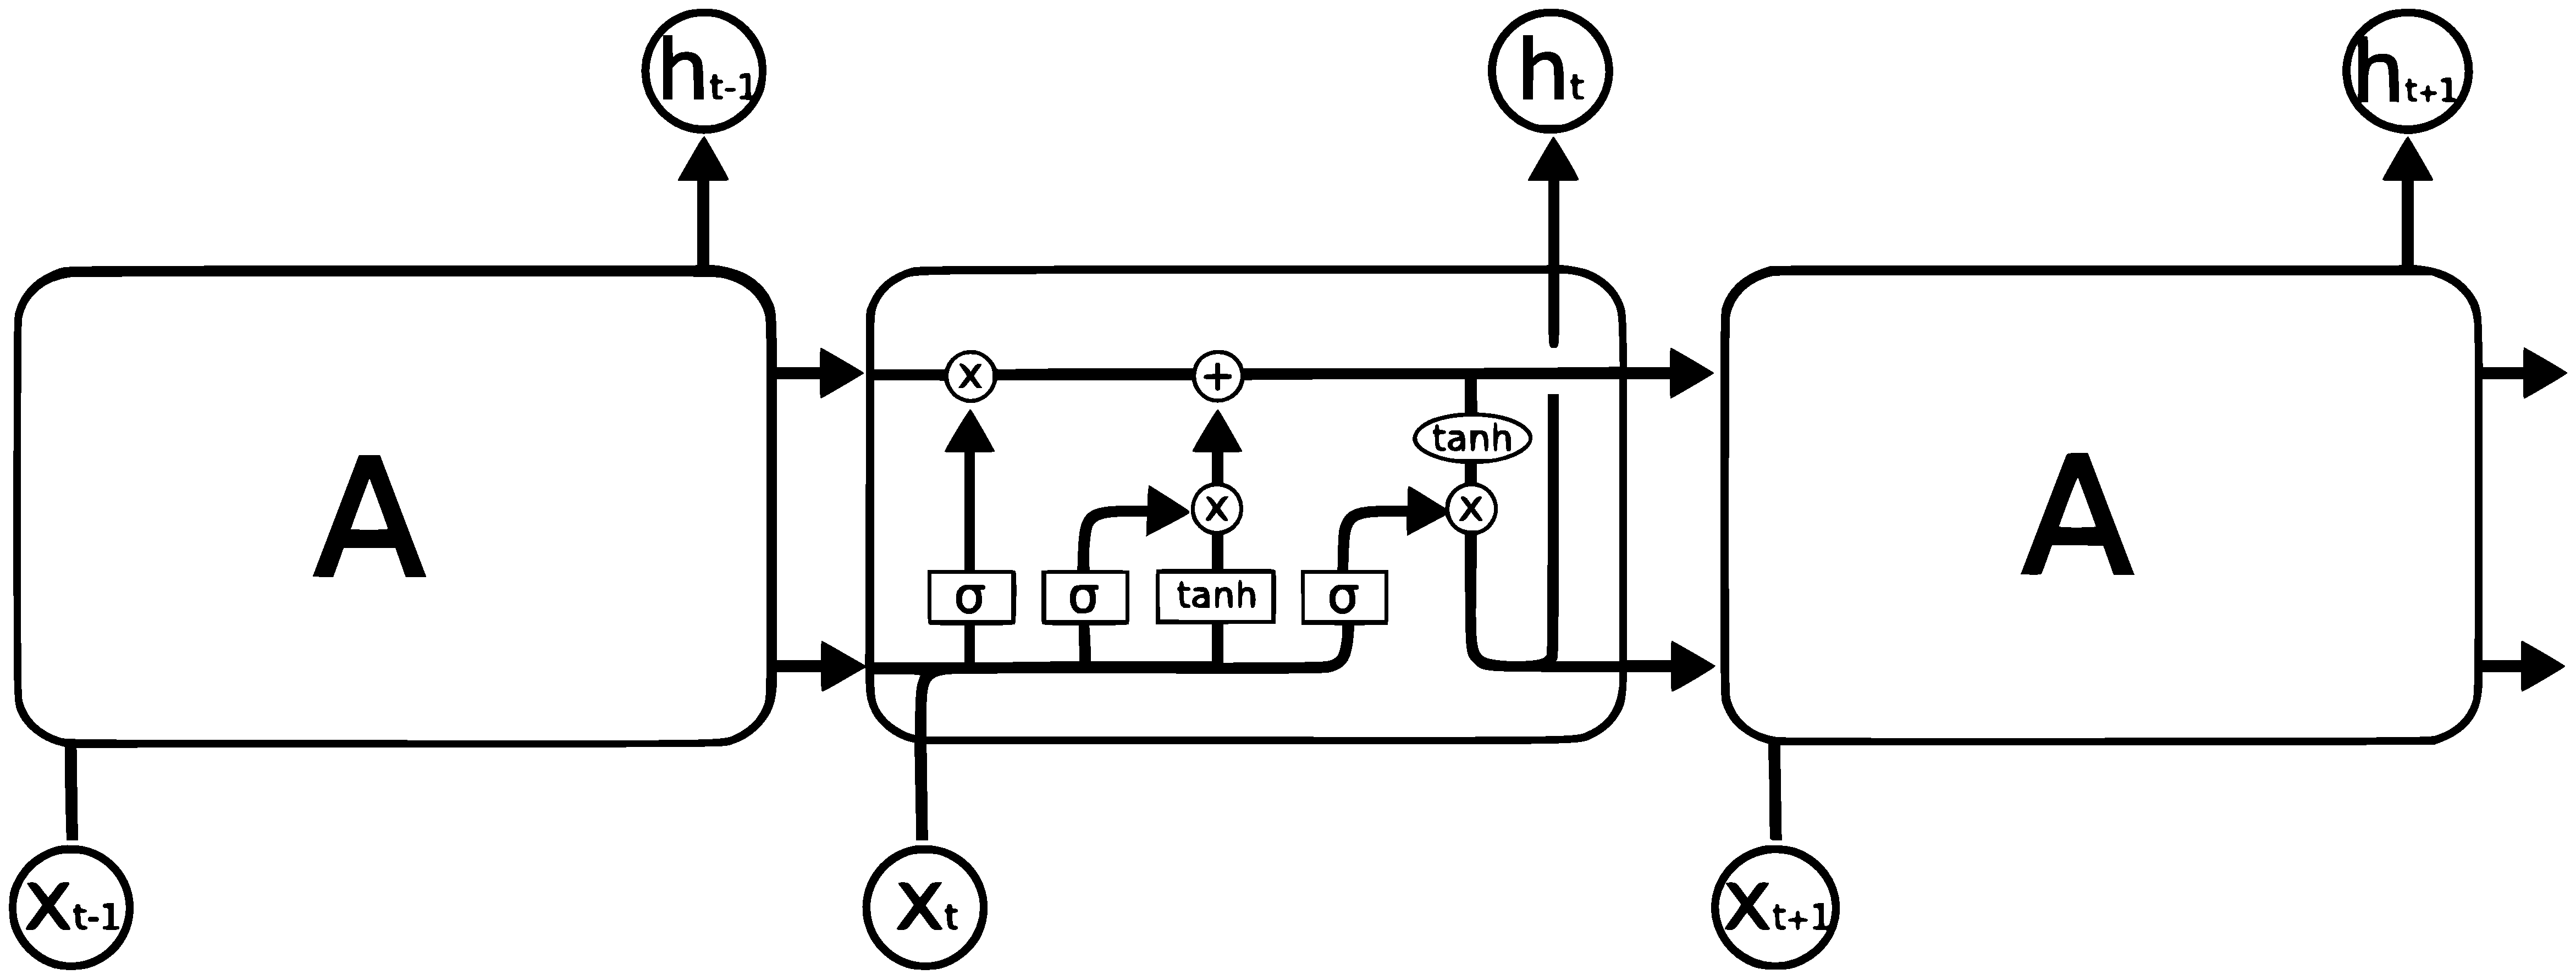
\includegraphics[width=\textwidth]    
    {machine_learning/01_Lstm_Diagram}
    \caption{LSTM Diagram.}
\end{figure}
From Figure \ref{fig:diagram_legend}, 
the lines represent vectors that pass
from the output of the previous node to the input of the current one. The circle denotes point wise operations, 
and the rectangle represents trained network layers.
\begin{figure}[H]
    \centering
    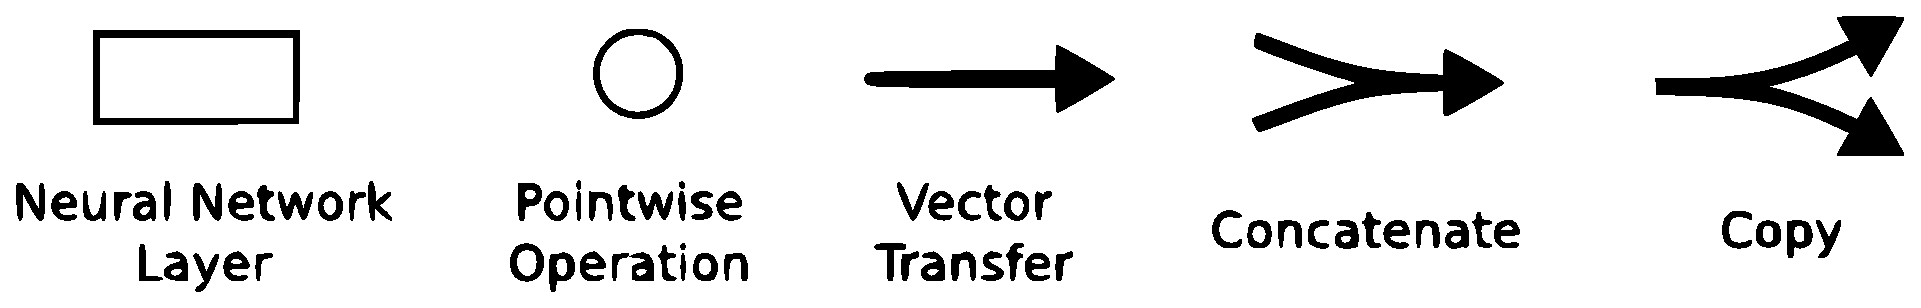
\includegraphics[width=\textwidth]        
    {machine_learning/02_Lstm_Notation}
    \caption{Diagram legend.}
    \label{fig:diagram_legend}
\end{figure}
A side by side description of each layer of an LSTM and
it`s mathematical formulation can be seen in the
following figures, where the dot represents matrix
multiplication.
The first layer represents the forget gate.
This is where we decide which information to keep and which to discard.
The layer outputs a value between zero and one for each input because of the sigmoid function
(represented as sigma in the equations below),
meaning that a value of zero represents data that will be
complicity erased and so forth, while an absolute value
of one represents data that will be left unchanged for
the next iteration.    
\begin{figure}[H]
    \centering
    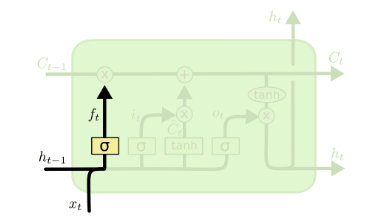
\includegraphics[width=0.5\textwidth]        
    {machine_learning/03_RForget}
    \caption{Forget Gate for concatenated inputs.}
    \label{fig:Forget}
\end{figure}
\begin{equation}
         f= \sigma(X.W_f+b_f) 
\end{equation}
Similar to the forget gate, the LSTM structure also uses an update gate, to add new information to the system.
As seen in Figure \ref{fig:Update}, the update gate generates the new values that will be used. This takes place by multiplying the update gate to the input layer, represented by $X`$ where a hyperbolic tangent is used as the activation function. This is given as an example, as the Rectified Linear Unit (ReLU) or the softmax activation work perfectly fine as well.  
From the above mentioned gates a new internal state C can be computed as:
\begin{equation}
	C_t= f * C_{t-1} + u*X` 
\end{equation}
Where the current state ($C_t$) is determined by what we want to forget ($f$), multiplied by the previous state ($C_t-1$) and added together with the update gate ($r$) times the input layer ($X`$).
\begin{figure}[H]
    \centering
        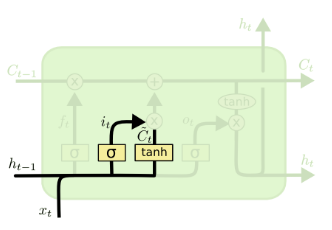
\includegraphics[width=0.5\textwidth]        
        {machine_learning/04_Update}
    		\caption{Update gate with the current state description.}
    		\label{fig:Update}
\end{figure}
\begin{equation}
	U= \sigma(X.W_u+b_u)
\end{equation}    
\begin{equation}     
	X`=\tanh(X.W_c+b_c)
\end{equation}
\begin{figure}[H]
    \centering
    		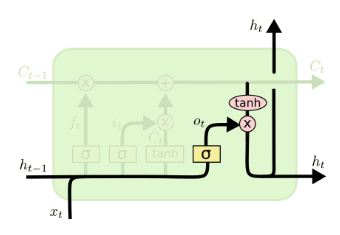
\includegraphics[width=0.5\textwidth]    					{machine_learning/05_Result}
    		\caption{Result gate added to the output function.}
    		\label{fig:Result}
\end{figure}
\begin{equation}
	r= \sigma(X.W_r+b_r) 
\end{equation}    
The third and last gate is the result gate ($r$), which uses the previous internal state of the LSTM to generate a new internal state.
As such, the output of the neural network can be written as:
\begin{equation}
	Y_t=\text{softmax}(H_t.W+b)
\end{equation}
%---------------------------------------------------
\subsection{Bidirectional networks}\label{sub:BiRNN}

Bidirectional Recurrent Neural Networks (BiRNN) are used to increase the 
input information available to the network. As data flows in one direction, standard neural networks have inherited restrictions where 
the future input cannot be accessed by the current state \cite{graves2005bidirectional}. Conversely,
BRNNs do not require their input data to be fixed. Furthermore, their 
future input information is available at the current state. This is done
by connecting two hidden layers of opposite directions to the same output.

For an input sequence like: $X=\left\{x_1,x_2,x_3,...,x_n \right\}$, a 
neural network computes the hidden vector layer 
$h=\left\{h_1,h_2,h_3,...,h_n \right\}$ and output vector 
$y=\left\{y_1,y_2,y_3,...,y_n \right\}$ by iterating over  $1<t<n$ to generate the following equations:
\begin{align}
h_t &= \sigma(W_{xh}*x_t + W_{hh}*h_{t-1} + b_h)\\
y_t &= W_{hy}*h_t + b_y
\end{align}

These equation expand on Section \ref{sec:ANN} and show how the neurons output a weighted sum of all the inputs and biases.
Because of the promising results given by simple LSTM networks, combining them with the benefits given by BRNN, the gates showcased in 
Subsection \ref{sub:LSTM} become:
\begin{align}
i_t &= \sigma(W_{xy} * x_t + W_{hi} * h_{t-1} + W_{ci} * c_{t-1} + b_i)
\\
f_t &= \sigma(W_{xf} * x_t + W_{hf} * h_{t-1} + W_{cf} * c_{t-1} + b_f) \\
c_t &= f_t * c_{t-1} + i_{t} * \tanh(W_{xc} * x_t + W_{hc} *  h_{t-1} + b_c)
\\
o_t &= \sigma(W_{xo} * x_t + W_{ho} * h_{t-1} + W_{co} * c_t +b_o))
\\
h_t &= o_t * \tanh(c_t)
\end{align}
Where i, f, o and c are the input gate, forget gate, output gate and cell activation vector. Because speech is a continuous action and entire utterances happen at once, simple RNNs fall behind in performance by only accessing previous information. Bidirectional RNNs process data in
two directions, with one layer iterating  forward (from t = 1 to n) and one layer iterating backwards (from t = n to 1), seen in Figure \ref{fig:BiRNN} \cite{graves2013hybrid}. As such, the forward layer is described in Equation \ref{eq:Forward} while the backwards layer is described in Equation \ref{eq:Backward} and the updated output layer, Equation \ref{eq:Output}, becomes:
\begin{align}
\overrightarrow{h}_t &= \sigma(W_{x\overrightarrow{h}} * x_t + W_{\overrightarrow{h}\overrightarrow{h}} * \overrightarrow{h}_{t-1}+ b_{\overrightarrow{h}}) \label{eq:Forward}
\\
\overleftarrow{h}_t &= \sigma(W_{x\overleftarrow{h}} * x_t + W_{\overleftarrow{h}\overleftarrow{h}} * \overleftarrow{h}_{t-1}+ b_{\overleftarrow{h}}) \label{eq:Backward}
\\
y_t &= W_{\overrightarrow{h}y} * \overrightarrow{h}_t + W_{\overleftarrow{h}y} * \overleftarrow{h}_t + b_y \label{eq:Output}
\end{align}

\begin{figure}[H]
	\centering
	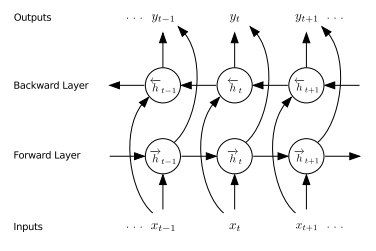
\includegraphics[width=0.75\textwidth]		
	{machine_learning/07_BiRNN}
	\caption{Visual representation of the hidden layers of one BiRNN}
	\label{fig:BiRNN}
\end{figure}
%---------------------------------------------------
\subsection{Dropout}

Dropout is a regularization technique that involves shooting the neurons.
It is applied after the activation function of each layer with the notable exception of the input and output layer.
A percentage is used to determine the number of neurons that will remain in the networks.
For example, a .75 pkeep value in the dropout function means that only 75 percent of the neurons will remain active during the training phase. \\\\\
For the testing phase, all the neurons have to be present, meaning that a value of one has to be given to the dropout function to ensure a high accuracy rating.
This helps the network understand the information it is given as it cannot presume that other neurons in the same layer have been activated and it prevents the network from just memorizing the values that were given as inputs.\\\\
The snippet of code below shows how dropout is used in TensorFlow for a layer of a neural network, where "pkeep" is the percentage of the neurons that will remain active and the call for the dropout is made after the activation function, in this case, the ReLU.
\begin{lstlisting}[language=Python, caption=Dropout for single network layer.]
pkeep = tf.palceholder(tf.float32)
YF = tf.nn.relu(tf.matmul(X, W)+ b)
Y = tf.nn.dropout(Yf, pkeep)
\end{lstlisting}
For a visual representation of a dropout rate given to a neural network, it can be seen Figure \ref{fig:.4_dropout_rate}.
A dropout rate of $40\%$ given to the neural network on the left hand side, which can be seen in the the neural network on the right hand side.
\begin{figure}[H]
	\centering
	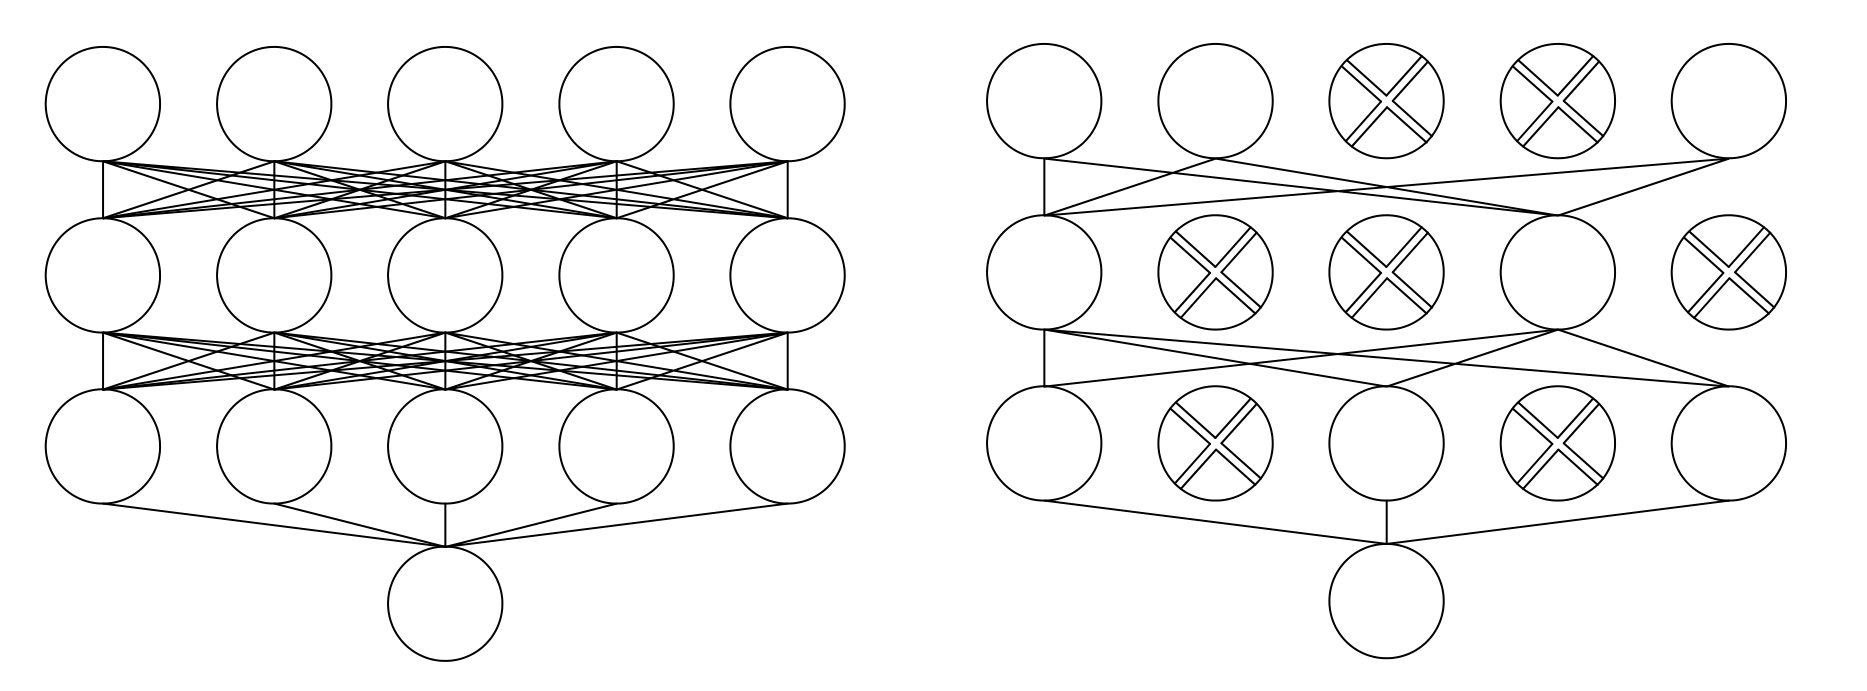
\includegraphics[width=\textwidth, height = 0.3\textheight]		
	{machine_learning/06_Dropoutpng}
	\caption{A $0.4$ dropout rate on a four layer network.}
	\label{fig:.4_dropout_rate}
\end{figure}

%---------------------------------------------------
\subsection{Batch normalisation}
Statistics can be computed for each batch that is fed to the neural network so the average and the standard deviation can be computed. After computing them, subtracting the average and dividing by the standard deviation rescales and re-enters the output. 
In the equation, epsilon is added to avoid numerical problems as dividing by zero.
\begin{equation}
    X= \dfrac{x - avg(x)}{stdev(x) + \epsilon} 
\end{equation}
The re-center and rescaling of the values can cause problems to
the network for cases where data needs to be squeezed over 
to one side of the spectrum.
To solve those cases, two degrees of freedom are added, 
$\alpha$ and $\beta$, for each neuron. 
By assigning the $\alpha$ value to the $stdev(x)$ and the
$\beta$ to $-avg(x)$ there will always be a case where the batch
normalized value of x can be reverted to the original value \cite{MonDieu}.
\begin{equation}
    BN(x) = \alpha * X + \beta
\end{equation}
Batch normalization (BN) is added as a layer before the activation function
because it makes use of the current weights and biases to
compute the average and standard deviation. Because of the new values added by BN,
biases are no longer useful.
The $\beta$ value can take the value of the bias if no better
values were found.
In contrast to the ReLU, when using a sigmoid,
the scale parameter has to be used to make sure that
the data fits in the useful part of the activation function.
A representation of how to choose the right coefficients is
given in Table \ref{tab:Parameters}.
\begin{table}[htbp]
\centering
    \caption{Parameters for different activation functions.}
    \begin{tabular}{l c c}
    \toprule
          & ReLU & Sigmoid \\\midrule
        Without BN &b & b  \\
        With BN & $\beta$ & $\alpha$, $\beta$  \\
    \bottomrule
    \end{tabular}
\label{tab:Parameters}
\end{table}

%---------------------------------------------------
\section{TensorFlow}
TensorFlow provides multiple Application Programming Interfaces
(APIs) for machine learning. 
The lowest level API "TensorFlow Core" provides complete programming control \cite{tensorflow2015-whitepaper}. 
For those who require fine levels of control over their models,
TensorFlow Core is a well-suited tool for the job. There are higher level APIs that are built on top of TensorFlow Core.
These higher level APIs are typically easier to learn and use than Tensorflow Core \cite{tensorflow2015-whitepaper}.
In addition, the higher level APIs such as "tf.estimator" helps with managing data sets, estimators,
training and inferences (testing your trained network),
as well as, making repetitive tasks easier and more consistent
\cite{tensorflow2015-whitepaper}.\\\\
The subsection below will start with TensorFlow Core. 
In order to gain an understanding of the basic principles that TensorFlow has to offer, a model shall be made. 
In the subsection after that, the same model will be implemented with tf.estimator. 
Knowing TensorFlow Core principles will give us a great mental model of how things are working internally when we use the more compact higher level API.

\subsection{Tensors}
The central unit of data in TensorFlow is the tensor. 
A tensor consists of a set of primitive values shaped into an array of any number of dimensions. 
A tensor's rank is its number of dimensions. 
Here are some examples of tensors:
\begin{lstlisting}[language=Python, caption=Tensor examples.]
3 # a rank 0 tensor; this is a scalar with shape []
[1.,2.,3.] # a rank 1 tensor; this is a vector with shape [3]
[[1.,2.,3.], [4., 5., 6.]] # a rank 2 tensor; a matrix with shape [2,3]
[[[1.,2.,3.]], [[7.,8.,9.]]] # a rank 3 tensor with shape [2,1,3]
\end{lstlisting} 

\subsection{TensorFlow Core}
Getting started with TensorFlow is done by using the import statement. 
This gives Python access to all of TensorFlow's classes,
methods and symbols. It is called by the following statement:
\begin{lstlisting}[language=Python, caption=Importing Tensorflow library.]
import tensorflow as tf
\end{lstlisting}
All the programs written with the help of TensorFlow core are built around computational graphs. 
They are a series of operations arranged into a graph and connected by nodes. 
To see the outcome of such a program, 
firstly the computational graph needs to be created and after that, it needs to be run. 
This provides a contrast to normal code written in python and to display this, 
the print function for a tensorflow constant is called bellow.
\begin{lstlisting}[language=Python, caption=Printing output without sess.run().]
node1 = tf.constant(3.0, dtype=tf.float32)
node2 = tf.constant(4.0) # also tf.float32 implicitly
print(node1, node2)

Output:
Tensor("Const:0", shape=(), dtype=float32)
Tensor("Const_1:0", shape=(), dtype=float32) 
\end{lstlisting}
As seen above, printing an element does not show the value that it holds and it rather shows the technical details behind,
such as the element being a constant of type float32.
To investigate the contents of any element in tensorflow,
an object of type session needs to be defined.
When the new object is run, a new session is generated and the content of the element can be seen.
All code written in tensorflow core follows this basic principle.
\begin{lstlisting}[language=Python, caption=Printing output with sess.run().]
sess = tf.Session()
print(sess.run([node1, node2]))

Output:
[3.0]
\end{lstlisting}
Other basic elements in tensorflow are
placeholders(tf.placeholder), they can be changed to accept external inputs and variables. Variables allow the system to
change its outputs while keeping the same inputs,
this allows the model to be trainable. 

\subsection{tf.train API}
The tf.train API holds optimizers that change each variable to minimize the loss function.
One of the simplest optimizers used to train neural networks is gradient descent.
Each variable is modified by the magnitude of the derivative of loss with respect to that variable.
Using a computer to gain these gradients is far less prone to error than doing it by hand.
Each of the gradients will point towards the minimum of the loss function and when solving for the gradient a step needs to be determined by the rate of change.
It is important to  have a small step as to not jump over the valley where the function takes its minimum value,
but in the beginning to reduce time and processing power a bigger step could be used.
One solution to this problem is to use a variable step input that changes as the gradients are determined.
TensorFlow can automatically produce derivatives given only a description of the model using the function tf.gradients.
For simplicity, optimizers typically do this for us.
\begin{lstlisting}[language=Python, caption=The gradient descent optimizer.]
optimizer = tf.train.GradientDescentOptimizer(0.01)
train = optimizer.minimize(loss)
sess.run(train)
\end{lstlisting}
The gradient descent optimizer takes an input, defined as 0.01 in the example above,
that represents the step input or the rate of change for the gradients.

\subsection{tf.estimator API}
%---------------------------------------------------
To simplify the procedure of machine learning,
tf.estimator can be used as a higher-level library within Tensorflow.
It helps the user with running training and evaluation loops, managing data sets and much more. 
Making the entire process of writing an algorithm and maintaining it be less tedious.
Although the estimator library has a set of predefined models to make things easier, a custom model can be created while keeping the high
level abstraction of the data set, training, and feeding.
A linear regression algorithm built with tf.estimator is included below to show how the library works \cite{Estimator}:
\begin{lstlisting}[language=Python, caption=Linear regression algorithm built with tf.estimator.]
import numpy as np
import tensorflow as tf

# Declare list of features. We only have one numeric feature. There are many
# other types of columns that are more complicated and useful.
feature_columns = [tf.feature_column.numeric_column("x", shape=[1])]

# An estimator is the front end to invoke training (fitting) and evaluation
# (inference). There are many predefined types like linear regression,
# linear classification, and many neural network classifiers and regressors.

# The following code provides an estimator that does linear regression.
estimator = tf.estimator.LinearRegressor(feature_columns=feature_columns)

# TensorFlow provides many helper methods to read and set up data sets.
# Here we use two data sets: one for training and one for evaluation
# We have to tell the function how many batches
# of data (num_epochs) we want and how big each batch should be.
x_train = np.array([1., 2., 3., 4.])
y_train = np.array([0., -1., -2., -3.])
x_eval = np.array([2., 5., 8., 1.])
y_eval = np.array([-1.01, -4.1, -7, 0.])
input_fn = tf.estimator.inputs.numpy_input_fn(
    {"x": x_train}, y_train, batch_size=4, num_epochs=None, shuffle=True)
train_input_fn = tf.estimator.inputs.numpy_input_fn(
    {"x": x_train}, y_train, batch_size=4, num_epochs=1000, shuffle=False)
eval_input_fn = tf.estimator.inputs.numpy_input_fn(
    {"x": x_eval}, y_eval, batch_size=4, num_epochs=1000, shuffle=False)

# We can invoke 1000 training steps by invoking the  method and passing the
# training data set.
estimator.train(input_fn=input_fn, steps=1000)

# Here we evaluate how well our model did.
train_metrics = estimator.evaluate(input_fn=train_input_fn)
eval_metrics = estimator.evaluate(input_fn=eval_input_fn)
print("train metrics: %r"% train_metrics)
print("eval metrics: %r"% eval_metrics)
\end{lstlisting}

%---------------------------------------------------
\section{Batch Size, Dropout and Learning Rate Comparison}
In order to gain a better understanding on how the different parameter values (batch size, dropout and learning rate) may affect the performance (training duration and test accuracy) of a neural network model, a small experiment was conducted.\\\\
This experiment consists of six test trials. For each test trial different parameter values were chosen, as shown in table \ref{tab:six_tests_tab}.
\begin{table}[H]
%Table with the six Tests
\centering
    \caption{Six tests with different Parameter values.}
    \begin{tabular}{| l | c | c | c | c | c | c | c |} 
    \hline
        Parameters & 
        Test1 -\tikzcircle[orange, fill=orange]{3pt}- &
        Test2 -\tikzcircle[blue, fill=blue]{3pt}- &
        Test3 -\tikzcircle[red, fill=red]{3pt}- &
        Test4 -\tikzcircle[lightblue, fill=lightblue]{3pt}- &
        Test5 -\tikzcircle[pink, fill=pink]{3pt}- &
        Test6 -\tikzcircle[turquoise, fill=turquoise]{3pt}- \\ 
    \hline
        Batch Size & 
        2 \hfill 2 \hfill 2 & 
        20 \hfill 20 \hfill 20 & 
        20 \hfill 20 \hfill 20 &
        20 \hfill 20 \hfill 20 &
        50 \hfill 20 \hfill 20 &
        50 \hfill 20 \hfill 20 \\
    \hline
        Dropout & 
        0.05 & 0.05 & 0.00 & 0.50 & 0.05 & 0.05 \\
    \hline
        Learning Rate & 
        0.001 & 0.001 & 0.001 & 0.001 & 0.001 & 0.010 \\
    \hline
    \end{tabular}
    \label{tab:six_tests_tab}
    %adding notes
    \raggedright{Batch Size: (train data, evaluation data, test data)} 
\end{table}
Note that the batch size is represented by the training, evaluation and testing data and will be represented this way
for all the following tables.\\\\
The tests were run on a model designed by the Silicon Valley
Data Science company, which is based on the TensorFlow
implementation of Baidu's DeepSpeech architecture on
the Mozilla' DeepSpeech repository.
The GitHub repositories (silicon-valley-data-science and Mozilla)
can be found respectively in the following citations:
\cite{rubashkin2017, mozilla2017}.
The model consists of a Bi-Directional Recurrent Neural Network
with three fully connected layers before it and a fully connected
layer with an activation layer after it.\\\\
The data used in the model referred above was a small set of WAV files consisting of recorded audio of the numbers:\\\\
$\left\{zero, one, two, three, four, five, six, seven, eight, nine \right\}$,\\\\
and their respective labels in text format. The data is separated into folders:
\begin{itemize}
    \item Train: train-clean-100-wav
    \item Test: test-clean-wav
    \item Dev: dev-clean-wav
\end{itemize}
In this section, the train and test results given in the following graphs and tables will be referred. However, for the interested
reader, all three train, test, and evaluation
results have been included in appendix \ref{ch:appBlabel} with slightly scaled up graphs for a more detailed analysis.
Here the goal is to visualize and compare the different graph curves and final results shown in the respective tables.
For consistency, all the tests are run for 25 Epochs. 

\subsection{Batch Size Test}
%-----------------------------------------------------
In this subsection three test from Table \ref{tab:six_tests_tab}  
will be used for the batch size test as shown in Table \ref{tab:batch_tests_tab}. For each trial test only the batch size parameter as been changed.

    %Batch Size Test table
    %-------------------------------------------------
\begin{table}[H]
\centering
    \caption{Three tests with different batch size values.}
    \begin{tabular}{| l | c | c | c | c |} 
    \hline
        Parameters & 
        Test1 -\tikzcircle[orange, fill=orange]{3pt}- &
        Test2 -\tikzcircle[blue, fill=blue]{3pt}- &
        Test5 -\tikzcircle[pink, fill=pink]{3pt}- \\
    \hline
        Batch Size & 
        2 \hfill 2 \hfill 2 & 
        20 \hfill 20 \hfill 20 & 
        50 \hfill 20 \hfill 20 \\
    \hline
        Dropout & 
        0.05 & 0.05 & 0.05 \\
    \hline
        Learning Rate & 
        0.001 & 0.001 & 0.001 \\ 
    \hline
    \end{tabular}
    \label{tab:batch_tests_tab}
\end{table}
    %-------------------------------------------------
The following graph (Fig. \ref{fig:batch_test_error_fig}) and
table (Tab. \ref{tab:batch_test_error_tab}) represent the error
rate for the test data set (the one that is used to test the
models accuracy after trainig). The results show that Test1 has
$\sim 13\%$ word error rate (WER) while Test2 and Test3 is
$\sim 0\%$ WER.

    %Batch Size Test error rate graph
    %-------------------------------------------------
\begin{figure}[H]
    %-------------------------------------------------
    \centering
    \includegraphics[width=\textwidth]        
    {machine_learning/graph_tests/batch_test/test_error_rate}
    \caption{Test error rate.}
    \label{fig:batch_test_error_fig}
\end{figure}
    %Batch Size Test error rate table
    %-------------------------------------------------
\begin{table}[H]
\centering
    \caption{Test error rate results.}
    \begin{tabular}{| l | c | c | c |}
    \hline
        Tests & Value & Epoch & Duration \\
    \hline
        Test1 -\tikzcircle[orange, fill=orange]{3pt}- &
        0.1308 & 25.00 & 0s\\
    \hline
        Test2 -\tikzcircle[blue, fill=blue]{3pt}- &
        0.000 & 25.00 & 0s\\
    \hline
        Test5 -\tikzcircle[pink, fill=pink]{3pt}- &
        0.000 & 25.00 & 0s\\
    \hline
    \end{tabular}
    \label{tab:batch_test_error_tab}
\end{table}
    %-------------------------------------------------
The following graph (Fig. \ref{fig:batch_train_error_fig}) and
table (Tab. \ref{tab:batch_train_error_tab}) represent the error
rate for the train data set (the one that is used to train the
model). The results show that Test1 took a duration of 
$\sim 1h 26m 13s$ for the trainig while Test2 and Test3 is 
$\sim 18m 50s$ and $\sim 14m 50s$ respectively. 
    %Batch Size training error rate graph
    %-------------------------------------------------
\begin{figure}[H]
    %-------------------------------------------------
    \centering
    \includegraphics[width=\textwidth]        
    {machine_learning/graph_tests/batch_test/train_error_rate}
    \caption{Training error rate.}
    \label{fig:batch_train_error_fig}
\end{figure}
    %Batch Size training error rate table
    %-------------------------------------------------
\begin{table}[H]
\centering
    \caption{Training error rate results.}
    \begin{tabular}{| l | c | c | c |}
    \hline
        Tests & Value & Epoch & Duration \\
    \hline
        Test1 -\tikzcircle[orange, fill=orange]{3pt}- &
        0.1148 & 24.00 & 1h 26m 13s\\
    \hline
        Test2 -\tikzcircle[blue, fill=blue]{3pt}- &
        9.5073e-4 & 24.00 & 18m 50s\\
    \hline
        Test5 -\tikzcircle[pink, fill=pink]{3pt}- &
        5.1858e-4 & 24.00 & 14m 50s\\
    \hline
    \end{tabular}
    \label{tab:batch_train_error_tab}
\end{table}    
    %-------------------------------------------------    
The final results show that Test1 with the smaller batch size took significantly longer to train and had the worst accuracy. However, Test3 with the larger batch size took the least time and had the same accuracy as Test2.
%-----------------------------------------------------

\subsection{Dropout Test}
In this subsection three test from Table \ref{tab:six_tests_tab}  
will be used for the batch size test as shown in Table \ref{tab:drop_tests_tab}. For each trial test, only the dropout
parameter has been changed.
    %Dropout Test table
    %-------------------------------------------------
\begin{table}[H]
\centering
    \caption{Three tests with different dropout values.}
    \begin{tabular}{| l | c | c | c | c |} 
    \hline
        Parameters & 
        Test2 -\tikzcircle[blue, fill=blue]{3pt}- &
        Test3 -\tikzcircle[red, fill=red]{3pt}- &
        Test4 -\tikzcircle[lightblue, fill=lightblue]{3pt}- \\
    \hline
        Batch Size & 
        20 \hfill 20 \hfill 20 & 
        20 \hfill 20 \hfill 20 &
        20 \hfill 20 \hfill 20 \\
    \hline
        Dropout & 
        0.05 & 0.00 & 0.50 \\
    \hline
        Learning Rate & 
        0.001 & 0.001 & 0.001 \\ 
    \hline
    \end{tabular}
    \label{tab:drop_tests_tab}
\end{table}
    %-------------------------------------------------
The following graph (Fig. \ref{fig:drop_test_error_fig}) and
table (Tab. \ref{tab:drop_test_error_tab}) represent the error
rate for the test data set. The results show that Test2 has
$\sim 0\%$ word error rate (WER) while Test3 and Test4 is
$\sim 3\%$ and $\sim 2\%$ WER respectively.
    %Dropout Test error rate graph
    %-------------------------------------------------
\begin{figure}[H]
    %-------------------------------------------------
    \centering
    \includegraphics[width=\textwidth]        
    {machine_learning/graph_tests/dropout_test/test_error_rate}
    \caption{Test error rate.}
    \label{fig:drop_test_error_fig}
\end{figure}
    %Dropout Test error rate table
    %-------------------------------------------------    
\begin{table}[H]
\centering
    \caption{Test error rate results.}
    \begin{tabular}{| l | c | c | c |}
    \hline
        Tests & Value & Epoch & Duration \\
    \hline
        Test2 -\tikzcircle[blue, fill=blue]{3pt}- &
        0.000 & 25.00 & 0s\\
    \hline
        Test3 -\tikzcircle[red, fill=red]{3pt}- &
        0.030 & 25.00 & 0s\\
    \hline
        Test4 -\tikzcircle[lightblue, fill=lightblue]{3pt}- &
        0.020 & 25.00 & 0s\\
    \hline
    \end{tabular}
    \label{tab:drop_test_error_tab}
\end{table}        
    %-------------------------------------------------
The following graph (Fig. \ref{fig:drop_train_error_fig}) and
table (Tab. \ref{tab:drop_train_error_tab}) represent the error
rate for the train data set. The results show that Test2 took a duration of $\sim 18m 50s$ while Test2 and Test3 took 
$\sim 18m 5s$ and $\sim 18m 10s$ respectively.
    %Dropout Training error rate graph
\begin{figure}[H]
    %-------------------------------------------------
    \centering
    \includegraphics[width=\textwidth]        
    {machine_learning/graph_tests/dropout_test/train_error_rate}
    \caption{Training error rate.}
    \label{fig:drop_train_error_fig}
\end{figure}
    %Dropout Training error rate table
    %-------------------------------------------------
\begin{table}[H]
\centering
    \caption{Training error rate results.}
    \begin{tabular}{| l | c | c | c |}
    \hline
        Tests & Value & Epoch & Duration \\
    \hline
        Test2 -\tikzcircle[blue, fill=blue]{3pt}- &
        9.5973e-4 & 24.00 & 18m 50s\\
    \hline
        Test3 -\tikzcircle[red, fill=red]{3pt}- &
        0.000 & 24.00 & 18m 5s\\
    \hline
        Test4 -\tikzcircle[lightblue, fill=lightblue]{3pt}- &
        6.3331e-3 & 24.00 & 18m 10s\\
    \hline
    \end{tabular}
    \label{tab:drop_train_error_tab}
\end{table}        
    %-------------------------------------------------
The final results show that Test3 with no dropout and Test4 with a high dropout of $50\%$ had a slightly faster training time, However, the test error rate was slightly worse than Test2 with a dropout of $5\%$. Overall all three tests performed very well. \todo{check dropout percentage}
%-----------------------------------------------------

\subsection{Learning Rate Test}
In this subsection two test from Table \ref{tab:six_tests_tab}  
will be used for the batch size test as shown in Table
\ref{tab:learning_tests_tab}. For each trial test, only the
learning rate parameter has been changed.
    %Learning Test table
    %-------------------------------------------------
\begin{table}[H]
\centering
    \caption{Two tests with different learning rate values.}
    \begin{tabular}{| l | c | c | c |} 
    \hline
        Parameters & 
        Test5 -\tikzcircle[pink, fill=pink]{3pt}- &
        Test6 -\tikzcircle[turquoise, fill=turquoise]{3pt}- \\ 
    \hline
        Batch Size & 
        50 \hfill 20 \hfill 20 &
        50 \hfill 20 \hfill 20 \\
    \hline
        Dropout & 0.05 & 0.05 \\
    \hline
        Learning Rate & 0.001 & 0.010 \\ 
    \hline
    \end{tabular}
    \label{tab:learning_tests_tab}
\end{table}
    %-------------------------------------------------
The following graph (Fig. \ref{fig:learning_test_error_fig}) and
table (Tab. \ref{tab:learning_test_error_tab}) represent the error rate for the test data set. The results show that Test5 has
$\sim 0\%$ word error rate (WER) while Test6 is $\sim 89\%$ WER.
    %Learning Test error rate graph
    %-------------------------------------------------
\begin{figure}[H]
    %-------------------------------------------------
    \centering
    \includegraphics[width=\textwidth]        
    {machine_learning/graph_tests/learning_rate_test/test_error_rate}
    \caption{Test error rate.}
    \label{fig:learning_test_error_fig}
\end{figure}
    %Learning Test error rate table
    %-------------------------------------------------
\begin{table}[H]
\centering
    \caption{Test error rate results.}
    \begin{tabular}{| l | c | c | c |}
    \hline
        Tests & Value & Epoch & Duration \\
    \hline
        Test5 -\tikzcircle[pink, fill=pink]{3pt}- &
        0.000 & 25.00 & 0s\\
    \hline
        Test6 -\tikzcircle[turquoise, fill=turquoise]{3pt}- &
        0.8992 & 25.00 & 0s\\
    \hline
    \end{tabular}
    \label{tab:learning_test_error_tab}
\end{table}        
    %-------------------------------------------------
The following graph (Fig. \ref{fig:learning_train_error_fig} and
table (Tab. \ref{tab:learning_train_error_tab}) represent the error rate for the train data set. The results show that Test5 took a duration of $\sim 14m 50s$ while Test6 took 
$\sim 12m 29s$.
    %Learning Training error rate graph
    %-------------------------------------------------
\begin{figure}[H]
    %-------------------------------------------------
    \centering
    \includegraphics[width=\textwidth]        
    {machine_learning/graph_tests/learning_rate_test/train_error_rate}
    \caption{Training error rate.}
    \label{fig:learning_train_error_fig}
\end{figure}
    %Learning Training error rate table
    %-------------------------------------------------
\begin{table}[H]
\centering
    \caption{Training error rate results.}
    \begin{tabular}{| l | c | c | c |}
    \hline
        Tests & Value & Epoch & Duration \\
    \hline
        Test5 -\tikzcircle[pink, fill=pink]{3pt}- &
        5.1858e-4 & 24.00 & 14m 50s\\
    \hline
        Test6 -\tikzcircle[turquoise, fill=turquoise]{3pt}- &
        0.9188 & 24.00 & 12m 29s\\
    \hline
    \end{tabular}
    \label{tab:learning_train_error_tab}
\end{table}        
    %-------------------------------------------------
The final results show that Test5 with no learning rate of 
$0.1\%$ outperformed Test6 with a learning rate of $1\%$ by a long shot. The graph clearly shows while training didn't really converge to zero at all, unlike Test5, meaning it didn't learn anything during training.
%----------------------------------------------------
\todo{write a summary about all this}